\chapter{Revised Plan}\label{ch:plan}

In light of our discoveries \todo{ $<$- wording, phrasing} on changing the type checker,
the project of the schedule has been updated to reflect the time needed to change the project,
seen in \autoref{fig:revisedplan}.

\begin{figure}
    \centering
    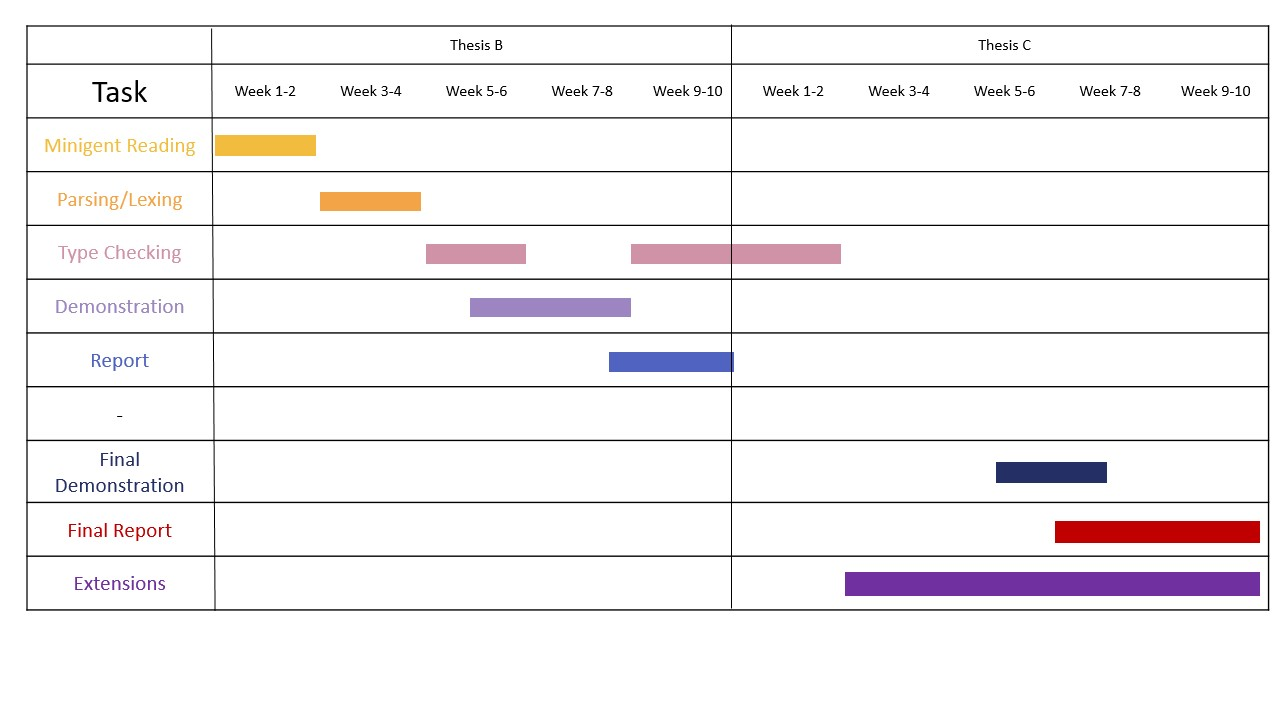
\includegraphics[height=0.50\textheight, angle=90]{content/revised_plan.jpg}
    \caption{The timeline for the project}
    \label{fig:revisedplan}
\end{figure}

Extra time has been allocated to update the type checking phase of Minigent in order to deal with
adding extra typechecking measure to \textsf{take} and \textsf{put}, in exchange of the time
needed to add type inference to remove \textsf{roll} and \textsf{unroll}. To complete this,
we must finalise the work in the type checker for automatically \textsf{roll}/\textsf{unroll} recursive type expressions
as explained in \autoref{sec:typecheckingprogress}.

As we no longer need to infer the use of \textsf{roll} and \textsf{unroll}, we have gained an extra
few weeks to work on the extensions of the project outlined in \autoref{sec:proposedextensions}.

The most important extension is to add primitive recursion detection for functions marked by
a \textsf{primrec} keyword, so that the programmer can get a guarantee from Minigent that
a function terminates before considering any kind of proof of termination.

This would allow programmers increased proof-concious development while writing Cogent code,
and upon integration with the Cogent embedding a potential termination proof for free for
functions that Cogent can guarantee are primitive recursive.

The primitive recursion extension is unbounded however, as writing an algorithm to detect primitive
recursion cannot cover all primitive recursive functions \todo{Is this true? I'm pretty sure I read
that there is no general algorithm to prove such a thing}, and thus can only cover more and more
functions inside the domain of primitive recursive functions.

\todo{Should I be talking about reasearch into this sort of stuff now? Or should I move it to the background and then reference
it here?}
\citet{AboutPrimrecAlgorithms}, in his paper on primitive recursive algorithms describes the
an inductive definition of primitive recursive functions via combinators on the natural numbers:

\theoremstyle{definition}
\begin{definition}
    \label{def:primrec}
    A function is \textit{primitive recursive} if it can be constructed using 
    a combination of the following combinators:

    \begin{itemize}
        \item 
            \textsf{O}, the \textit{null} or \textit{constant} combinator that takes zero arguemnts.
        \item 
            \textsf{Succ}, the \textit{successor} combinator that takes one argument, and returns the successor
            of that argument.
        \item 
            \textsf{$\pi^n_i$}, the \textit{projection} combinator that takes $n \geq 1$ arguments and returns
            the $i$'th argument, where $1 \leq i \leq n$.
        \item 
            \textsf{$S^n_m(f, g_1, g_2, \dots, g_n)$}, the \textit{composition} combinator, where $f$ and $g_{1..n}$ are 
            primitive recursive combinators that take $n$ and $m$ arguments respectfully, such that 
                $$S^n_m(f, g_1, g_2, \dots, g_n) = f(g_1(x_1, \dots, x_m), \dots, g_n(x_1, \dots, x_m))$$
        \item 
            \textsf{$Rec(b,s)$}, where $b$ and $s$ are primitive recursive combinators that take
            $n + 1$ arguments and $n + 2$ arguments respectfully is the \textit{recursion}
            combinator with base case $b$ and recursive step $n$.
    \end{itemize}
\end{definition}

In addition to a means to translate our Cogent and Minigent programs into the above combinators,
we seek a method to map expressions to natural numbers that the above combinators can
operate on. Constructing this mapping correctly is a proof that our function is primitive recursive and
therefore terminates, otherwise however gives us no information about our function.

Alternatively or in conjunction with the primitive recursive approach, we may consider using
structurally recursive methods as discussed by \citet{StrucrecStructures} and \citet{PredicateStructrec}.
In this case our goal is to find a \textit{termination order} upon which our functions terminate --- An ordering
where each recursive call operates on arguments that are `smaller' than the previous. 
As we don't have infinite objects in our recursive types due to their strictly positive condition, 
we know that are datatypes are finite in size, so functions that are  structurally recursive must
merely descend on the structure of the datatype, as measured by our termination order.

\citet{PredicateStructrec} talks in particular about \textit{structural ordering}, by measuring term size in
terms of constructors. They describe two axioms to measue this order, the first being given
a term $e$ and a constructor $C$, the transitive closure of:
$$
    e < C (\dots, e, \dots)
$$
And for measuring the size of function expressions, given a function $f$ of type $\alpha \longrightarrow \tau$,
and an argument $a$ of type $\alpha$:
$$
    f\; a \leq f
$$
Where the justification for this comes from set theory --- as a function is represented as the set of all pairs of
arguments and results, the result of one function application ($f\; a$) is less than or equal to the set containing
all possible results ($f$).

\todo{lexicographical ordering}